\documentclass[twoside]{book}

% Packages required by doxygen
\usepackage{fixltx2e}
\usepackage{calc}
\usepackage{doxygen}
\usepackage[export]{adjustbox} % also loads graphicx
\usepackage{graphicx}
\usepackage[utf8]{inputenc}
\usepackage{makeidx}
\usepackage{multicol}
\usepackage{multirow}
\PassOptionsToPackage{warn}{textcomp}
\usepackage{textcomp}
\usepackage[nointegrals]{wasysym}
\usepackage[table]{xcolor}

% Font selection
\usepackage[T1]{fontenc}
\usepackage[scaled=.90]{helvet}
\usepackage{courier}
\usepackage{amssymb}
\usepackage{sectsty}
\renewcommand{\familydefault}{\sfdefault}
\allsectionsfont{%
  \fontseries{bc}\selectfont%
  \color{darkgray}%
}
\renewcommand{\DoxyLabelFont}{%
  \fontseries{bc}\selectfont%
  \color{darkgray}%
}
\newcommand{\+}{\discretionary{\mbox{\scriptsize$\hookleftarrow$}}{}{}}

% Page & text layout
\usepackage{geometry}
\geometry{%
  a4paper,%
  top=2.5cm,%
  bottom=2.5cm,%
  left=2.5cm,%
  right=2.5cm%
}
\tolerance=750
\hfuzz=15pt
\hbadness=750
\setlength{\emergencystretch}{15pt}
\setlength{\parindent}{0cm}
\setlength{\parskip}{3ex plus 2ex minus 2ex}
\makeatletter
\renewcommand{\paragraph}{%
  \@startsection{paragraph}{4}{0ex}{-1.0ex}{1.0ex}{%
    \normalfont\normalsize\bfseries\SS@parafont%
  }%
}
\renewcommand{\subparagraph}{%
  \@startsection{subparagraph}{5}{0ex}{-1.0ex}{1.0ex}{%
    \normalfont\normalsize\bfseries\SS@subparafont%
  }%
}
\makeatother

% Headers & footers
\usepackage{fancyhdr}
\pagestyle{fancyplain}
\fancyhead[LE]{\fancyplain{}{\bfseries\thepage}}
\fancyhead[CE]{\fancyplain{}{}}
\fancyhead[RE]{\fancyplain{}{\bfseries\leftmark}}
\fancyhead[LO]{\fancyplain{}{\bfseries\rightmark}}
\fancyhead[CO]{\fancyplain{}{}}
\fancyhead[RO]{\fancyplain{}{\bfseries\thepage}}
\fancyfoot[LE]{\fancyplain{}{}}
\fancyfoot[CE]{\fancyplain{}{}}
\fancyfoot[RE]{\fancyplain{}{\bfseries\scriptsize Generated by Doxygen }}
\fancyfoot[LO]{\fancyplain{}{\bfseries\scriptsize Generated by Doxygen }}
\fancyfoot[CO]{\fancyplain{}{}}
\fancyfoot[RO]{\fancyplain{}{}}
\renewcommand{\footrulewidth}{0.4pt}
\renewcommand{\chaptermark}[1]{%
  \markboth{#1}{}%
}
\renewcommand{\sectionmark}[1]{%
  \markright{\thesection\ #1}%
}

% Indices & bibliography
\usepackage{natbib}
\usepackage[titles]{tocloft}
\setcounter{tocdepth}{3}
\setcounter{secnumdepth}{5}
\makeindex

% Hyperlinks (required, but should be loaded last)
\usepackage{ifpdf}
\ifpdf
  \usepackage[pdftex,pagebackref=true]{hyperref}
\else
  \usepackage[ps2pdf,pagebackref=true]{hyperref}
\fi
\hypersetup{%
  colorlinks=true,%
  linkcolor=blue,%
  citecolor=blue,%
  unicode%
}

% Custom commands
\newcommand{\clearemptydoublepage}{%
  \newpage{\pagestyle{empty}\cleardoublepage}%
}

\usepackage{caption}
\captionsetup{labelsep=space,justification=centering,font={bf},singlelinecheck=off,skip=4pt,position=top}

%===== C O N T E N T S =====

\begin{document}

% Titlepage & ToC
\hypersetup{pageanchor=false,
             bookmarksnumbered=true,
             pdfencoding=unicode
            }
\pagenumbering{alph}
\begin{titlepage}
\vspace*{7cm}
\begin{center}%
{\Large Arbutus }\\
\vspace*{1cm}
{\large Generated by Doxygen 1.8.14}\\
\end{center}
\end{titlepage}
\clearemptydoublepage
\pagenumbering{roman}
\tableofcontents
\clearemptydoublepage
\pagenumbering{arabic}
\hypersetup{pageanchor=true}

%--- Begin generated contents ---
\chapter{Hierarchical Index}
\section{Class Hierarchy}
This inheritance list is sorted roughly, but not completely, alphabetically\+:\begin{DoxyCompactList}
\item \contentsline{section}{Element}{\pageref{class_element}}{}
\begin{DoxyCompactList}
\item \contentsline{section}{Button}{\pageref{class_button}}{}
\begin{DoxyCompactList}
\item \contentsline{section}{Slider}{\pageref{class_slider}}{}
\begin{DoxyCompactList}
\item \contentsline{section}{Vertical\+Slider}{\pageref{class_vertical_slider}}{}
\end{DoxyCompactList}
\end{DoxyCompactList}
\item \contentsline{section}{Splitter}{\pageref{class_splitter}}{}
\item \contentsline{section}{Viewport}{\pageref{class_viewport}}{}
\end{DoxyCompactList}
\item \contentsline{section}{G\+UI}{\pageref{class_g_u_i}}{}
\item \contentsline{section}{G\+U\+I\+Style}{\pageref{class_g_u_i_style}}{}
\item of\+Base\+App\begin{DoxyCompactList}
\item \contentsline{section}{of\+App}{\pageref{classof_app}}{}
\end{DoxyCompactList}
\item \contentsline{section}{Splitter\+Child}{\pageref{struct_splitter_child}}{}
\item \contentsline{section}{Trigger\+Visual\+Action}{\pageref{class_trigger_visual_action}}{}
\end{DoxyCompactList}

\chapter{Class Index}
\section{Class List}
Here are the classes, structs, unions and interfaces with brief descriptions\+:\begin{DoxyCompactList}
\item\contentsline{section}{\hyperlink{class_button}{Button} }{\pageref{class_button}}{}
\item\contentsline{section}{\hyperlink{class_element}{Element} }{\pageref{class_element}}{}
\item\contentsline{section}{\hyperlink{class_g_u_i}{G\+UI} }{\pageref{class_g_u_i}}{}
\item\contentsline{section}{\hyperlink{class_g_u_i_style}{G\+U\+I\+Style} }{\pageref{class_g_u_i_style}}{}
\item\contentsline{section}{\hyperlink{classof_app}{of\+App} }{\pageref{classof_app}}{}
\item\contentsline{section}{\hyperlink{class_slider}{Slider} }{\pageref{class_slider}}{}
\item\contentsline{section}{\hyperlink{class_splitter}{Splitter} }{\pageref{class_splitter}}{}
\item\contentsline{section}{\hyperlink{struct_splitter_child}{Splitter\+Child} }{\pageref{struct_splitter_child}}{}
\item\contentsline{section}{\hyperlink{class_trigger_visual_action}{Trigger\+Visual\+Action} }{\pageref{class_trigger_visual_action}}{}
\item\contentsline{section}{\hyperlink{class_vertical_slider}{Vertical\+Slider} }{\pageref{class_vertical_slider}}{}
\item\contentsline{section}{\hyperlink{class_viewport}{Viewport} }{\pageref{class_viewport}}{}
\end{DoxyCompactList}

\chapter{Class Documentation}
\hypertarget{class_app_g_u_i}{}\section{App\+G\+UI Class Reference}
\label{class_app_g_u_i}\index{App\+G\+UI@{App\+G\+UI}}
\subsection*{Public Member Functions}
\begin{DoxyCompactItemize}
\item 
\mbox{\Hypertarget{class_app_g_u_i_a99335b7a84b20086736ae186fa27baa8}\label{class_app_g_u_i_a99335b7a84b20086736ae186fa27baa8}} 
void {\bfseries setup} (string resources\+Path)
\item 
\mbox{\Hypertarget{class_app_g_u_i_abf7a3105a2391c3a075a79d8876fadb1}\label{class_app_g_u_i_abf7a3105a2391c3a075a79d8876fadb1}} 
Element $\ast$ {\bfseries get\+Main\+Output\+Viewport} ()
\item 
\mbox{\Hypertarget{class_app_g_u_i_a84734dc3dcfec0f390c538b6cd092e45}\label{class_app_g_u_i_a84734dc3dcfec0f390c538b6cd092e45}} 
Element $\ast$ {\bfseries get\+Layer\+Preview\+And\+Info} (unsigned int layer\+Number)
\item 
\mbox{\Hypertarget{class_app_g_u_i_a260cf32da70bde9ea8e3d4375db41930}\label{class_app_g_u_i_a260cf32da70bde9ea8e3d4375db41930}} 
Element $\ast$ {\bfseries get\+Layer\+Viewport} (unsigned int layer\+Number)
\item 
\mbox{\Hypertarget{class_app_g_u_i_ad95d80ea59eea6ea82680015effffbab}\label{class_app_g_u_i_ad95d80ea59eea6ea82680015effffbab}} 
Element $\ast$ {\bfseries get\+Visual\+Instance\+At\+Layer} (unsigned int layer\+Number)
\end{DoxyCompactItemize}


The documentation for this class was generated from the following files\+:\begin{DoxyCompactItemize}
\item 
src/\+Arbutus/App\+G\+U\+I.\+hpp\item 
src/\+Arbutus/App\+G\+U\+I.\+cpp\end{DoxyCompactItemize}

\hypertarget{class_controls_group}{}\section{Controls\+Group Class Reference}
\label{class_controls_group}\index{Controls\+Group@{Controls\+Group}}
\subsection*{Public Member Functions}
\begin{DoxyCompactItemize}
\item 
\mbox{\Hypertarget{class_controls_group_ab5821ef9cf29cb1c338dee833997e8be}\label{class_controls_group_ab5821ef9cf29cb1c338dee833997e8be}} 
\mbox{\hyperlink{class_controls_group_ab5821ef9cf29cb1c338dee833997e8be}{Controls\+Group}} ()
\begin{DoxyCompactList}\small\item\em Contructor. \end{DoxyCompactList}\item 
\mbox{\Hypertarget{class_controls_group_a191f5c1d1b6b05c4b78448d9249e295a}\label{class_controls_group_a191f5c1d1b6b05c4b78448d9249e295a}} 
\mbox{\hyperlink{class_controls_group_a191f5c1d1b6b05c4b78448d9249e295a}{$\sim$\+Controls\+Group}} ()
\begin{DoxyCompactList}\small\item\em Destructor. \end{DoxyCompactList}\item 
\mbox{\Hypertarget{class_controls_group_ac2a18a055b26b18ce3ab1bc7aa085f7b}\label{class_controls_group_ac2a18a055b26b18ce3ab1bc7aa085f7b}} 
void \mbox{\hyperlink{class_controls_group_ac2a18a055b26b18ce3ab1bc7aa085f7b}{set}} (json data)
\begin{DoxyCompactList}\small\item\em ... \end{DoxyCompactList}\item 
\mbox{\Hypertarget{class_controls_group_a1ca5952b0e990590cff420be29679420}\label{class_controls_group_a1ca5952b0e990590cff420be29679420}} 
void \mbox{\hyperlink{class_controls_group_a1ca5952b0e990590cff420be29679420}{set\+Parent\+Element}} (Element $\ast$\+\_\+element)
\begin{DoxyCompactList}\small\item\em ... \end{DoxyCompactList}\item 
\mbox{\Hypertarget{class_controls_group_a591c730dd207bd39152f550c6ff01f94}\label{class_controls_group_a591c730dd207bd39152f550c6ff01f94}} 
void \mbox{\hyperlink{class_controls_group_a591c730dd207bd39152f550c6ff01f94}{set\+Properties}} (Properties $\ast$\+\_\+properties)
\begin{DoxyCompactList}\small\item\em ... \end{DoxyCompactList}\item 
\mbox{\Hypertarget{class_controls_group_aefd772a7034081fbcce964f96ae20947}\label{class_controls_group_aefd772a7034081fbcce964f96ae20947}} 
Element $\ast$ \mbox{\hyperlink{class_controls_group_aefd772a7034081fbcce964f96ae20947}{add\+Float}} (json \+\_\+element\+Data, string key)
\begin{DoxyCompactList}\small\item\em ... \end{DoxyCompactList}\item 
\mbox{\Hypertarget{class_controls_group_a0fce3a0d0d3f1a7f86fe614b50c091d4}\label{class_controls_group_a0fce3a0d0d3f1a7f86fe614b50c091d4}} 
Element $\ast$ \mbox{\hyperlink{class_controls_group_a0fce3a0d0d3f1a7f86fe614b50c091d4}{add\+Button\+Group}} (json \+\_\+element\+Data, string key)
\begin{DoxyCompactList}\small\item\em ... \end{DoxyCompactList}\item 
\mbox{\Hypertarget{class_controls_group_a9cc5691e2f7376342627d4e23554f338}\label{class_controls_group_a9cc5691e2f7376342627d4e23554f338}} 
Element $\ast$ \mbox{\hyperlink{class_controls_group_a9cc5691e2f7376342627d4e23554f338}{add\+Toggle\+Button\+Group}} (json \+\_\+element\+Data, string key)
\begin{DoxyCompactList}\small\item\em ... \end{DoxyCompactList}\item 
\mbox{\Hypertarget{class_controls_group_a38a87e6db9f03df1fc4a53831f27bdb5}\label{class_controls_group_a38a87e6db9f03df1fc4a53831f27bdb5}} 
void \mbox{\hyperlink{class_controls_group_a38a87e6db9f03df1fc4a53831f27bdb5}{set\+Controls\+Display\+Order}} (json \+\_\+display\+Order)
\begin{DoxyCompactList}\small\item\em ... \end{DoxyCompactList}\item 
json \mbox{\hyperlink{class_controls_group_a603fcb3050fd34c148a0bb4e85890474}{dump\+Json}} ()
\begin{DoxyCompactList}\small\item\em returns a json with the information of the control group \end{DoxyCompactList}\item 
\mbox{\Hypertarget{class_controls_group_a98939ab75fed4fb25d0ff769c871c87c}\label{class_controls_group_a98939ab75fed4fb25d0ff769c871c87c}} 
void {\bfseries update\+Parent\+Rect} (Element $\ast$last\+Added\+Element)
\end{DoxyCompactItemize}


\subsection{Member Function Documentation}
\mbox{\Hypertarget{class_controls_group_a603fcb3050fd34c148a0bb4e85890474}\label{class_controls_group_a603fcb3050fd34c148a0bb4e85890474}} 
\index{Controls\+Group@{Controls\+Group}!dump\+Json@{dump\+Json}}
\index{dump\+Json@{dump\+Json}!Controls\+Group@{Controls\+Group}}
\subsubsection{\texorpdfstring{dump\+Json()}{dumpJson()}}
{\footnotesize\ttfamily json Controls\+Group\+::dump\+Json (\begin{DoxyParamCaption}{ }\end{DoxyParamCaption})}



returns a json with the information of the control group 

\begin{DoxyReturn}{Returns}
a json variable 
\end{DoxyReturn}


The documentation for this class was generated from the following files\+:\begin{DoxyCompactItemize}
\item 
src/\+Arbutus/Controls\+Group.\+hpp\item 
src/\+Arbutus/Controls\+Group.\+cpp\end{DoxyCompactItemize}

\hypertarget{classof_app}{}\section{of\+App Class Reference}
\label{classof_app}\index{of\+App@{of\+App}}


{\ttfamily \#include $<$of\+App.\+h$>$}

Inheritance diagram for of\+App\+:\begin{figure}[H]
\begin{center}
\leavevmode
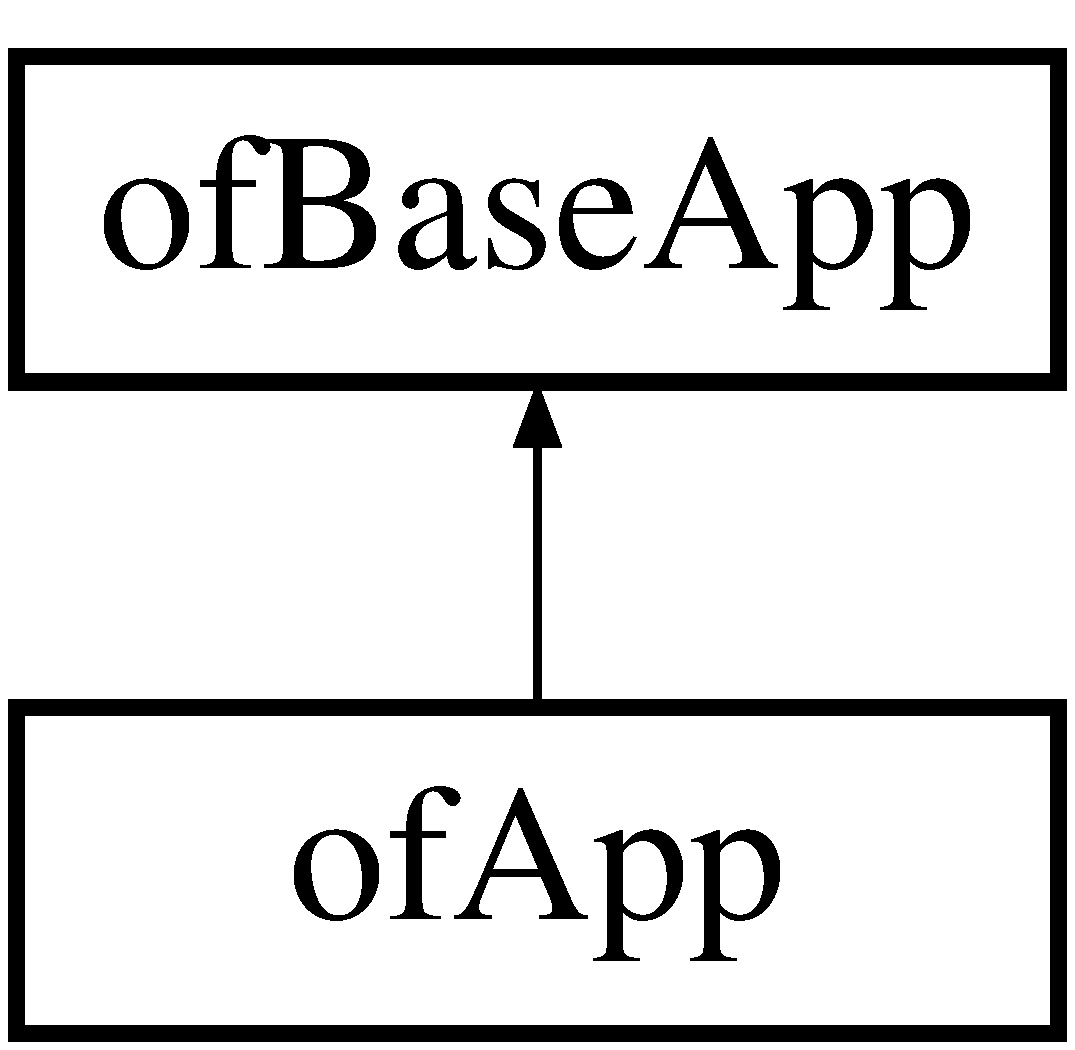
\includegraphics[height=2.000000cm]{classof_app}
\end{center}
\end{figure}
\subsection*{Public Member Functions}
\begin{DoxyCompactItemize}
\item 
\mbox{\Hypertarget{classof_app_af68eaa1366244f7a541cd08e02199c12}\label{classof_app_af68eaa1366244f7a541cd08e02199c12}} 
void {\bfseries setup} ()
\item 
\mbox{\Hypertarget{classof_app_afef41ea4aee5a22ea530afba33ae7a7b}\label{classof_app_afef41ea4aee5a22ea530afba33ae7a7b}} 
void {\bfseries update} ()
\item 
\mbox{\Hypertarget{classof_app_a75dd45437b9e317db73d8daef1ad49f8}\label{classof_app_a75dd45437b9e317db73d8daef1ad49f8}} 
void {\bfseries draw} ()
\item 
\mbox{\Hypertarget{classof_app_a957d3197364bbac8e67eaa4f15b28ad3}\label{classof_app_a957d3197364bbac8e67eaa4f15b28ad3}} 
void {\bfseries key\+Pressed} (int key)
\item 
\mbox{\Hypertarget{classof_app_aa1503a87453bcfdd395fe4acca5d91a0}\label{classof_app_aa1503a87453bcfdd395fe4acca5d91a0}} 
void {\bfseries key\+Released} (int key)
\item 
\mbox{\Hypertarget{classof_app_a158b41a606310db4633fdb817b21047c}\label{classof_app_a158b41a606310db4633fdb817b21047c}} 
void {\bfseries mouse\+Moved} (int x, int y)
\item 
\mbox{\Hypertarget{classof_app_a1ec53d1be799dc275806ff6c6548cd83}\label{classof_app_a1ec53d1be799dc275806ff6c6548cd83}} 
void {\bfseries mouse\+Dragged} (int x, int y, int button)
\item 
\mbox{\Hypertarget{classof_app_a2c2ea9c160231e55424dfd98466ef27d}\label{classof_app_a2c2ea9c160231e55424dfd98466ef27d}} 
void {\bfseries mouse\+Pressed} (int x, int y, int button)
\item 
\mbox{\Hypertarget{classof_app_aa3131f1554fc49eaa9ee0f284e48129b}\label{classof_app_aa3131f1554fc49eaa9ee0f284e48129b}} 
void {\bfseries mouse\+Released} (int x, int y, int button)
\item 
\mbox{\Hypertarget{classof_app_ae4dc1ec1513dcbe48bc78a5e4c3fac0f}\label{classof_app_ae4dc1ec1513dcbe48bc78a5e4c3fac0f}} 
void {\bfseries window\+Resized} (int w, int h)
\item 
\mbox{\Hypertarget{classof_app_aada5a79556321801567752a0e5a69bda}\label{classof_app_aada5a79556321801567752a0e5a69bda}} 
void {\bfseries drag\+Event} (of\+Drag\+Info drag\+Info)
\item 
\mbox{\Hypertarget{classof_app_a885672a72340a5e998af1d16718dc766}\label{classof_app_a885672a72340a5e998af1d16718dc766}} 
void {\bfseries got\+Message} (of\+Message msg)
\item 
\mbox{\Hypertarget{classof_app_a6ee1a7af6a715c6448f9769ff22cbabc}\label{classof_app_a6ee1a7af6a715c6448f9769ff22cbabc}} 
void {\bfseries gui\+Test001} ()
\item 
\mbox{\Hypertarget{classof_app_ad561e567741c5979497091b4ce6c1517}\label{classof_app_ad561e567741c5979497091b4ce6c1517}} 
void {\bfseries gui\+Test002} ()
\end{DoxyCompactItemize}


\subsection{Detailed Description}


The documentation for this class was generated from the following files\+:\begin{DoxyCompactItemize}
\item 
src/\+Arbutus/of\+App.\+h\item 
src/\+Arbutus/of\+App.\+cpp\end{DoxyCompactItemize}

\hypertarget{class_secundary_window_app}{}\section{Secundary\+Window\+App Class Reference}
\label{class_secundary_window_app}\index{Secundary\+Window\+App@{Secundary\+Window\+App}}
Inheritance diagram for Secundary\+Window\+App\+:\begin{figure}[H]
\begin{center}
\leavevmode
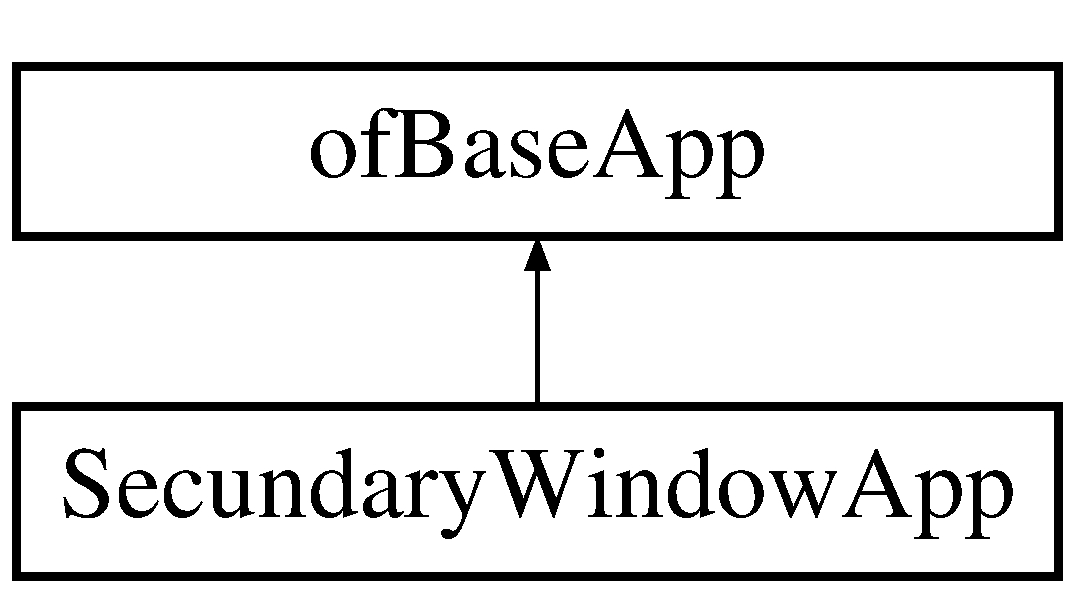
\includegraphics[height=2.000000cm]{class_secundary_window_app}
\end{center}
\end{figure}
\subsection*{Public Member Functions}
\begin{DoxyCompactItemize}
\item 
\mbox{\Hypertarget{class_secundary_window_app_af541b1d4d0f27d1eb8115af53c0fa41c}\label{class_secundary_window_app_af541b1d4d0f27d1eb8115af53c0fa41c}} 
void {\bfseries draw} ()
\item 
\mbox{\Hypertarget{class_secundary_window_app_a7109dc6edd44c48abd71a1a8d22a242a}\label{class_secundary_window_app_a7109dc6edd44c48abd71a1a8d22a242a}} 
void {\bfseries set\+Window} (shared\+\_\+ptr$<$ of\+App\+Base\+Window $>$ \+\_\+window)
\item 
\mbox{\Hypertarget{class_secundary_window_app_abf4df7c0359364a14e04ceaed4871b59}\label{class_secundary_window_app_abf4df7c0359364a14e04ceaed4871b59}} 
shared\+\_\+ptr$<$ of\+App\+Base\+Window $>$ {\bfseries get\+Window} ()
\end{DoxyCompactItemize}


The documentation for this class was generated from the following file\+:\begin{DoxyCompactItemize}
\item 
src/\+Arbutus/Windows.\+hpp\end{DoxyCompactItemize}

\hypertarget{class_windows}{}\section{Windows Class Reference}
\label{class_windows}\index{Windows@{Windows}}
\subsection*{Public Member Functions}
\begin{DoxyCompactItemize}
\item 
\mbox{\Hypertarget{class_windows_a038f74c39cb3fdaa40fb10d5095bdb92}\label{class_windows_a038f74c39cb3fdaa40fb10d5095bdb92}} 
void {\bfseries add} (shared\+\_\+ptr$<$ of\+App\+Base\+Window $>$ main\+Window)
\end{DoxyCompactItemize}


The documentation for this class was generated from the following files\+:\begin{DoxyCompactItemize}
\item 
src/\+Arbutus/Windows.\+hpp\item 
src/\+Arbutus/Windows.\+cpp\end{DoxyCompactItemize}

%--- End generated contents ---

% Index
\backmatter
\newpage
\phantomsection
\clearemptydoublepage
\addcontentsline{toc}{chapter}{Index}
\printindex

\end{document}
